

\documentclass{article}
\usepackage[english]{babel}
\usepackage[utf8]{inputenc}
\usepackage{amsmath}
\usepackage{amsfonts}
\usepackage{amssymb}
\usepackage{graphicx}
\usepackage[left=2cm, right=2cm, top=2cm, bottom=2cm]{geometry}

\title{\textbf{Prethermalization in one-dimensional quantum many-body systems with confinement}}

\author{Divyansh Wangnue}
\date{}

\begin{document}
\maketitle
\begin{abstract} 
Unconventional nonequilibrium phases with restricted correlation spreading and slow entanglement growth have been proposed to emerge in systems with confined excitations, calling their thermalization dynamics into question. Here, we show that in confined systems the thermalization dynamics after a quantum quench instead exhibits multiple stages with well separated time scales. As an example, we consider the confined Ising spin chain, in which domain walls in the ordered phase form bound states reminiscent of mesons. The system first relaxes towards a prethermal state, described by a Gibbs ensemble with conserved meson number. The prethermal state arises from rare events in which mesons are created in close vicinity, leading to an avalanche of scattering events. Only at much later times a true thermal equilibrium is achieved in which the meson number conservation is violated by a mechanism akin to the Schwinger effect. The discussed prethermalization dynamics is directly relevant to generic one-dimensional, many-body systems with confined excitations.
 \end{abstract}





\section{Overview}
\paragraph{Introduction}
Nonequilibrium states of quantum many-body systems play an important role in various fields of physics, including cosmology and condensed matter. Of particular interest is the time evolution of interacting quantum many-body systems that are well isolated from their environment. This research has been fueled by the progress in engineering coherent and interacting quantum many-body systems which made it possible to experimentally study unconventional relaxation dynamics. A recent interest is to explore phenomena from high-energy physics with synthetic quantum systems in a controlled way; for example lattice gauge theories have been realized and phenomena akin to quark confinement have been explored with great emphasis on the atypical nonequilibrium features of confined systems. Confinement strongly affects the relaxation dynamics of the system, leading to unconventional spreading of correlations and slow entanglement growth\cite{abc} with striking signatures in the energy spectrum reminicent of quantum scars. In spite of many efforts, a proper characterization of the full many-body dynamics and thermalization\cite{def} in confined systems remaines elusive so far.
\begin{equation}
O_t= \delta T  + \zeta ^ 2+ \pi /4 
\end{equation}
\paragraph{Context} 
An archetypical model to study confinement phenomena in condensed-matter settings is the Ising model with both transverse and longitudinal magnetic fields. In this model, domain walls—interpreted as quarks—are pairwise confined into mesons by a weak longitudinal field; see Fig. 1a. A key feature of the model is the long lifetime of mesons, ascribed to a strong suppression of the Schwinger mechanism\cite{ghi}, which creates new quarks from the energy stored in the confining force and viceversa. Hence, except for some fine-tuned regimes mesons are stable excitations. Due to the approximate conservation of the meson number, various exotic dynamical phenomena have been proposed, including Wannier-Stark localization\cite{jkl} and time crystals\cite{mno}. Even though the realization of these phenomena does not require particular fine tuning, they arise in a regime in which interactions between mesons are extremely unlikely. The few-meson scattering has been recently considered  but so far, apart from special limits\cite{pqr} the full many-body dynamics of confined systems has not been addressed. Irrespective of these exciting effects, the Ising model with longitudinal and transverse fields is non-integrable19 and features a Wigner-Dyson level statistics of the eigenenergies\cite{stu}.





\begin{itemize}
    \item  Hence, one would expect on general grounds that the system thermalizes at late times and interactions between mesons can become relevant. Given this wealth of unconventional nonequilibrium phenomena and the discrepancy with the expected thermalization in non-integrable models, it is important to understand the mechanisms of relaxation and their timescales.
    \item This research has been fueled by the progress in engineering coherent and interacting quantum many-body systems which made it possible to experimentally study unconventional relaxation dynamics
\end{itemize}







\begin{table}
\centering
\caption{\label{tab1} Energy Release (kJ)/mol .} 
\begin{tabular}{cccc}
\hline
Situation1 & Situation2 & Situation3 & Situation4 \\
\hline
577.71 & 871.7 & 86,1565.11 & 635.34\\
89.1 & 69.14 & 70.17 & 54.34\\
\hline
\end{tabular}
\end{table}


\begin{figure}
\centering
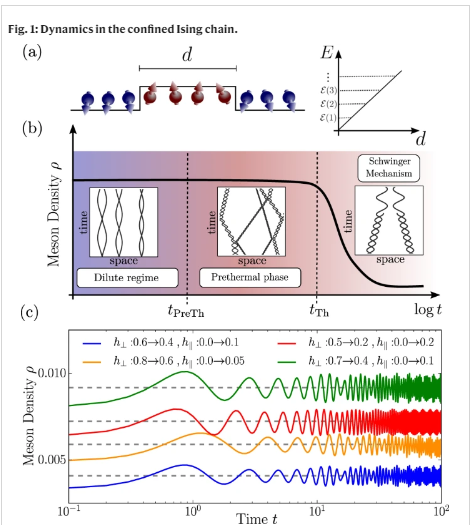
\includegraphics[scale=1]{thermoimg}
\caption{\label{fig1}Dynamics in the confined Ising chain}
\end{figure}

\begin{figure}
\centering
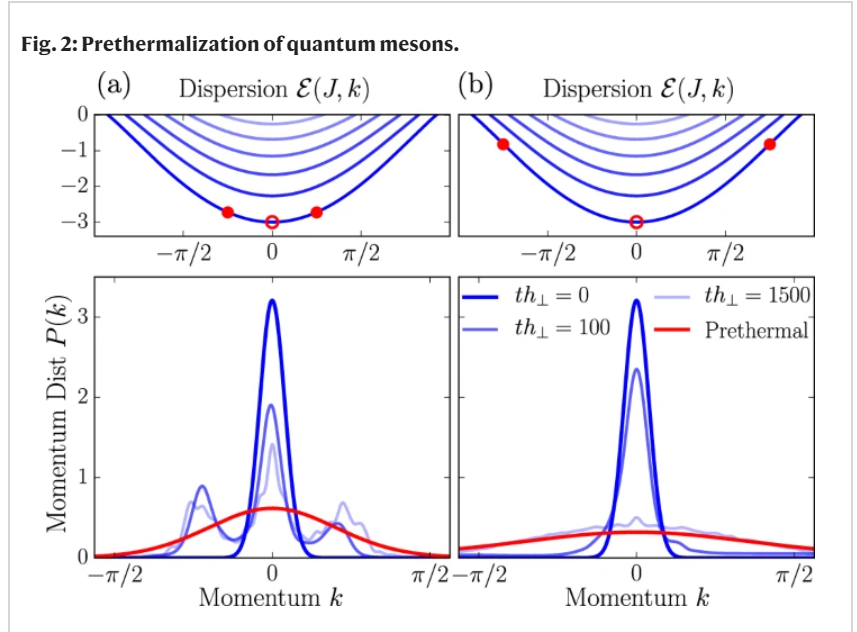
\includegraphics[scale=0.5]{secondimg}
\caption{\label{fig2}Prethermalization of quantum mesons}
\end{figure}

\begin{figure}
\centering
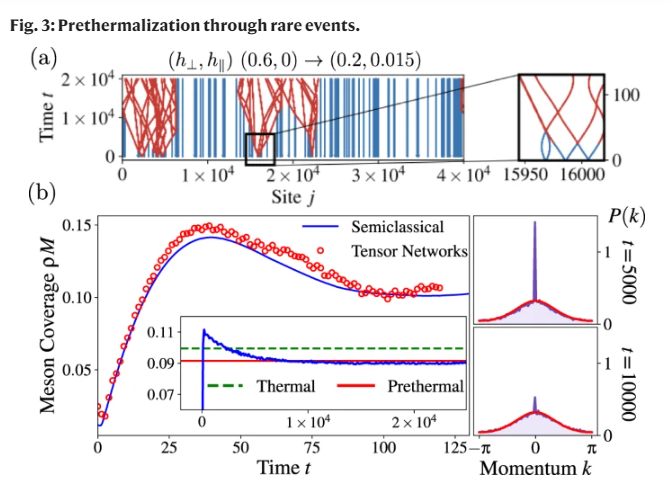
\includegraphics[width=0.8\textwidth]{thirdimg}
\caption{\label{fig3}Fig. 3: Prethermalization through rare events..}
\end{figure}



\section{Method}
Describe the methods used to create the dataset, including the following sub-headings:
\paragraph{Steps} The series of procedures followed to produce the dataset. This should include any source data used, as well as software and instrumentation involved.
\paragraph{Sampling strategy} If relevant, please outline the sampling strategy used to produce the data.
\paragraph{Quality control} If applicable. Please list the methods used for quality control in the production of the data (i.e., steps taken to normalize the data).

\section{Dataset Discussion}
Confined spin chains exhibit an intriguing multi-stage thermalization dynamics. We show that not the Schwinger mechanism is responsible for activating transport, but rather rare events in which two mesons are generated in their vicinity lead to a prethermal regime, that can be understood as a thermal gas of mesons. The different mechanism ensures the separation of timescales and the existence of a prethermal regime. The prethermalization time can be greatly reduced by considering quench protocols that create mesons with non-zero velocity. This, for example, can be realized with spatially modulated pulses of the transverse field \cite{h} (Supplementary information for details on the confining dynamics; characterization of the prethermal state; initialization of moving mesons by staggered field pulses; further information on details of numerical simulations.).

\section{Reuse Potential}
Please describe the ways in which your data could be reused by other researchers both within and outside of your field. For example, this might include aggregation, further analysis, reference, validation, teaching or collaboration. This section should also include limitations to, or potential barriers for reuse.

\section*{Acknowledgements}
We thank S. Scopa and P. Calabrese for collaboration on closely related topics and A. Lerose for useful discussions. We acknowledge support from the Deutsche Forschungsgemeinschaft (DFG, German Research Foundation) under Germany’s Excellence Strategy–EXC–2111–390814868, TRR80 and DFG grants No. KN1254/1-2 and No. KN1254/2-1, the European Research Council (ERC) under the European Union’s Horizon 2020 research and innovation programme (grant agreement No. 851161), as well as the Munich Quantum Valley, which is supported by the Bavarian state government with funds from the Hightech Agenda Bayern Plus.
\section*{Funding Statement}
Open Access funding enabled and organized by Projekt DEAL.

\section*{Competing interests} 
The authors declare no competing interests.


\begin{thebibliography}{8}
	\bibitem{abc} Schweizer, C. et al. Floquet approach to z2 lattice gauge theories with ultracold atoms
	\bibitem{def} Martinez, E. A. et al. Real-time dynamics of lattice gauge theories with a few-qubit
	\bibitem{ghi} Görg, F. et al. Realization of density-dependent peierls phases to engineer quantized
	\bibitem{jkl} Yang, B. et al. Observation of gauge invariance in a 71-site bose-hubbard quantum simulator
	\bibitem{mno} Mil, A. et al. A scalable realization of local u(1) gauge invariance in cold atomic mixtures.
	\bibitem{pqr} Satzinger, K. J. et al. Realizing topologically ordered states on a quantum processor.
	\bibitem{stu} Semeghini, G. et al. Probing topological spin liquids on a programmable quantum
	\bibitem{h} Tan, W. L. et al. Domain-wall confinement and dynamics in a quantum simulator.

\end{thebibliography} 

\end{document}